\documentclass[10pt,letter]{article}
\usepackage{amssymb,graphicx,amsmath,mathtools,ifthen,textcomp,enumerate,units,cancel}
\usepackage[margin=1.5in]{geometry}
\usepackage[T1]{fontenc}
\usepackage{tikz}
\numberwithin{equation}{section}
\newcommand{\problemdivider}{\begin{center}\large \bf\ldots\ldots\ldots\ldots\ldots\ldots\end{center}}
\newcommand{\subproblemdivider}{\begin{center}\large \bf\ldots\ldots\end{center}}
\newcommand{\pdiv}{\problemdivider}
\newcommand{\spdiv}{\subproblemdivider}
\newcommand{\ba}{\begin{align*}}
\newcommand{\ea}{\end{align*}}
\newcommand{\rt}{\right}
\newcommand{\lt}{\left}
\newcommand{\bp}{\begin{problem}}
\newcommand{\ep}{\end{problem}}
\newcommand{\bsp}{\begin{subproblem}}
\newcommand{\esp}{\end{subproblem}}
\newcommand{\bssp}{\begin{subsubproblem}}
\newcommand{\essp}{\end{subsubproblem}}
\newcommand{\atag}[1]{\addtocounter{equation}{1}\label{#1}\tag{\arabic{section}.\alph{subsection}.\alph{equation}}}
\newcommand{\btag}[1]{\addtocounter{equation}{1}\label{#1}\tag{\arabic{section}.\alph{equation}}}
\newcommand{\ctag}[1]{\addtocounter{equation}{1}\label{#1}\tag{\arabic{equation}}}
\newcommand{\unts}[1]{\ \text{#1}}
\newcommand{\textop}[1]{\operatorname{#1}}
\newcommand{\textopl}[1]{\operatornamewithlimits{#1}}
\newcommand{\prt}{\partial}
\newcommand{\pderi}[3]{\frac{\prt^{#3}#1}{\prt #2^{#3}}}
\newcommand{\deri}[3]{\frac{d^{#3}#1}{d #2^{#3}}}
\newcommand{\del}{\vec\nabla}
\newcommand{\exval}[1]{\langle #1\rangle}
\newcommand{\bra}[1]{\langle #1|}
\newcommand{\ket}[1]{|#1\rangle}
\newcommand{\ham}{\mathcal{H}}
\newcommand{\arr}{\mathfrak{r}}

\newcommand{\bsm}{\lt(\begin{smallmatrix}}
\newcommand{\esm}{\end{smallmatrix}\rt)}
\newcommand{\bpm}{\begin{pmatrix}}
\newcommand{\epm}{\end{pmatrix}}
\newcommand{\bdet}{\lt|\begin{smallmatrix}}
\newcommand{\edet}{\end{smallmatrix}\rt|}

\newcommand{\bs}[1]{\boldsymbol{#1}}
\newcommand{\uvec}[1]{\bs{\hat{#1}}}

\newcommand{\qed}{\hfill$\Box$}

\def\thesection{\textbf{\arabic{section}}}
\def\thesubsection{\textbf{\thesection.\alph{subsection}.}}
\def\thesubsubsection{\textbf{\alph{subsubsection}.}}

\makeatletter
\newenvironment{problem}[1]{\ifthenelse{\arabic{section}>0}{\pdiv}{}\@startsection
       {section}
       {1}
       {0em}
       {0em}
       {0em}
       {\pagebreak[3]}{\bf #1}\hspace{3mm}}
       {}
\newenvironment{subproblem}[1]{\ifthenelse{\arabic{subsection}>0}{\spdiv}{}\@startsection
       {subsection}
       {2}
       {0em}
       {0em}
       {0em}
       {\pagebreak[3]}{\it #1}.}
       {}
\newenvironment{subsubproblem}{\@startsection
       {subsubsection}
       {3}
       {0em}
       {0em}
       {0em}
       {\pagebreak[3]}}
       {}
\makeatother


\begin{document}
\noindent\textbf{\textsc{HapASeg}}\\
\noindent\textsc{Julian Hess}\\
\noindent 19 February 2021\\

\section{Intro}

Consider a set $\mathcal{S}$ of phased SNPs on haplotypes $\mathcal{A}$ and $\mathcal{B}$. SNP $i$ assigned to $\mathcal{A}$ has alternate read count $a_i$ and reference read count $b_i$, while SNP $j$ assigned to $\mathcal{B}$ has alternate read count $b_j$ and reference read count $a_j$. We can express the allelic imbalance $f$ of $\mathcal{S}$ in terms of the relative fraction of $\mathcal{A}$, which we call the ``haplotypic imbalance.'' In a diploid region of the genome, $f\approx 1/2$. In a triploid region with two copies of $\mathcal{A}$ and one copy of $\mathcal{B}$, $f\approx 2/3$.

Assuming only aleatoric uncertainty, the likelihood of the haplotypic imbalance $f$ for all SNPs in $\mathcal{S}$ is
\begin{align*}
\mathcal{L}(f|\mathcal{S}) &= \prod_{i\in\mathcal{S}} f^{a_i} (1 - f)^{b_i}\\
&= f^{\sum_{i\in\mathcal{S}} a_i}(1-f)^{\sum_{i\in\mathcal{S}} b_i}\\
&\equiv f^{A_\mathcal{S}}(1-f)^{B_\mathcal{S}}\btag{As}
%&\propto \textop{beta}\lt(1 + \textstyle\sum_{i\in\mathcal{S}} a_i, 1 + \sum_{i\in\mathcal{S}}  b_i\rt)\\
%&\equiv f\sim\textop{beta}(1 + A_\mathcal{S}, 1 + B_\mathcal{S})
\end{align*}
where $A_\mathcal{S}$ and $B_\mathcal{S}$ are the total read counts respectively assigned to $\mathcal{A}$ and $\mathcal{B}$ within segment $\mathcal{S}$. Since the SNPs are ordered along a chromosome, we can parameterize $\mathcal{S}$ in terms of the disjoint intervals defining each segment. Denote the genomic position of SNP $i$ as $x_i$, and the set of all SNPs as $\mathcal{X}$. For a given half-open genomic interval $[s_j,e_j)$, with $s_{j+1}=e_j$ and $s_1=1$, we have
\begin{align*}
\mathcal{L}(f_j,[s_j,e_j)|\mathcal{X})=\prod_{\mathclap{\{i|x_i\in [s_j, e_j)\}}} f_j^{a_i}(1 - f_j)^{b_i}
\end{align*}
which is equivalent to \eqref{As} above. Marginalizing out $f_j$ yields
\begin{align*}
\mathcal{L}([s_j,e_j)|\mathcal{X})&=\int_0^1 df_j\,\prod_{\mathclap{\{i|x_i\in [s_j, e_j)\}}} f_j^{a_i}(1 - f_j)^{b_i}\\
&= \beta(A_{\mathcal{S}_j}+1, B_{\mathcal{S}_j}+1)
\end{align*}
where $\beta$ is the beta function.

Our goal is to find a good allelic segmentation. This requires finding the optimal partition of all SNPs, i.e.\ the optimal set of $\{[s,e)\}$ that maximizes the marginal likelihood
\begin{align*}
\mathcal{L}(\{[s,e)\}|\mathcal{X})=\prod_j \mathcal{L}([s_j,e_j)|\mathcal{X}).
\end{align*}
Unfortunately, for $N$ total SNPs, the total number of possible partitions is $2^N$. Luckily, the space of partitions is amenable to sampling via MCMC. While this won't give us the exact optimal partition, it gives us something even better: the posterior probability of segmentations.

\section{MCMC}

Initially, each SNP belongs to its own segment. At random, we pick two adjacent segments and probabilistically merge them according to the Metropolis criterion:
\begin{align*}
\textop{Pr}(\underbrace{[s_j,e_j),[s_{j+1},e_{j+1})}_{S}\to \underbrace{[s_j,e_{j+1})}_{S^\ast}) = \min\lt\{1,\frac{\mathcal{M}(S^\ast)q(S|S^\ast)}{\mathcal{M}(S)q(S^\ast|S)}\rt\},\btag{metro}
\end{align*}
where marginal likelihoods are
\begin{align*}
\mathcal{M}(S^\ast) &= \beta(\underbrace{\textstyle\sum_{\{i|x_i\in [s_j, e_{j+1})\}}a_i}_{A_{[s_j,e_{j+1})}},\underbrace{\textstyle\sum_{\{i|x_i\in [s_j, e_{j+1})\}}b_i}_{B_{[s_j,e_{j+1})}})\btag{psum_1}\\
\mathcal{M}(S) &= \beta(A_{[s_j,e_j)},B_{[s_j,e_j)})\times \beta(A_{[s_{j+1},e_{j+1})},B_{[s_{j+1},e_{j+1})}).\btag{psum_2}
\end{align*}
We can also split segments of length $>1$. Rather than picking a breakpoint within the segment at random, we probabilistically tailor our proposal distribution. For each position $k\in [s_j,e_j)$, we compute
\begin{align*}
\mathcal{L}_j(k) = \beta(A_{[s_j,k)},B_{[s_j,k)})\times\beta(A_{[k,e_j)},B_{[k,e_j)}),\btag{psum_3}
\end{align*}
and propose picking $k$ as the breakpoint with probability $p_j(k)=\mathcal{L}_j(k)/\sum_k \mathcal{L}_j(k)$. Our proposal distributions are
\begin{align*}
q(S|S^\ast) = \frac{p_j(k)}{N} \qquad q(S^\ast|S) = \frac{1}{N-1}
\end{align*}
where $N$ is the total number of segments at the current MCMC iteration.

The overall MCMC procedure is:
\begin{enumerate}
\item Initialize each SNP to belong to its own segment.
\item With equal probability, pick whether to attempt a merge or split this iteration.
\item If we choose to merge, uniformly pick segment $j$ at random from 1 to $N-1$. Probabilistically merge it with segment $j+1$ with probability defined in \eqref{metro}.
\item If we choose to split, uniformly pick $j$ at random from 1 to $N$, propose a breakpoint within $j$ via \eqref{psum_3}, and accept the proposal with probability defined as the reciprocal of \eqref{metro}. Proposing a breakpoint at the end of the segment is equivalent to not accepting any proposal at all and leaving the chain as-is.
\item A given state of the chain constitutes a sample $\psi_i$ from the overall distribution of segmentations, $\Psi$. We iterate the chain until it is burned-in, then iterate some more until a sufficient number of samples $\psi_1,\dots,\psi_n\sim\Psi$ have been collected. Because the chain moves slowly between iterations (each iteration only modifies a single segment), we ``thin'' the chain and only save every $n$th sample ($n\sim 100$). In the future, we might want to adjust the thinning amount to reflect the average number of segments $\bar{N}_s$ at a given point in the chain, since we expect each $\bar{N}_s$ iterations will modify every single segment.
\end{enumerate}

The MCMC is extremely fast, since each iteration only involves computing partial sums in \eqref{psum_1}, \eqref{psum_2}, and \eqref{psum_3} which can be memoized between iterations. In theory, storing all possible partial sums would require $O(N^2)$ space, but in practice we only ever need blocks close to the diagonal, so the partial sum matrix can be stored sparse, with space complexity $O(\bar{N}_s\bar{B}^2)\ll O(N^2)$, where $\bar{N}_s$ is the average number of segments and $\bar{B}$ the average length of each segment. The MCMC is also efficiently parallelized: the most compute-intensive phase is at the beginning when each SNP belongs to its own segment. Blocks of adjacent SNPs are burned-in in parallel, which are then concatenated post burnin to sample the final segmentation posterior. During this step, each chromosome arm can be run in parallel, since we do not expect reliable phasing across the centromere.

\subsection{SNP pruning}

We optionally propose a third operation during each iteration: SNP pruning. Within a given segment, some SNPs' haplotypic imbalance $a_i/(a_i+b_i)$ can differ considerably from the true haplotypic imbalance of the segment, whether due to random chance or systematic bias (e.g., mapping issues, poor base qualities, etc.)

We can prune these SNPs from a segment, using an MCMC step similar to splitting a segment. For the $k$th SNP in the $j$th segment $\mathcal{S}_j$, we compute the marginal likelihood of the segment minus SNP $k$:
\begin{align*}
\mathcal{M}^{-}_j(k) = \beta(\underbrace{A_{[s_j,e_j)} - a_k}_{A^{-k}_{[s_j,e_j)}}, \underbrace{B_{[s_j,e_j)} - b_k}_{B^{-k}_{[s_j,e_j)}})\times\beta(a_k, b_k).
\end{align*}
Note that this is extremely similar to the likelihood of splitting a segment given in \eqref{psum_3}, with the ``segment'' being split out the single SNP $k$, which can be anywhere within $j$.

If $k$ had already been removed from $j$, the marginal likelihood of adding it back is
\begin{align*}
\mathcal{M}^{+}_j(k) = \beta(A^{-k}_{[s_j,e_j)} + a_k, B^{-k}_{[s_j,e_j)} + b_k).
\end{align*}

The posterior ratio for removing $k$ is
\begin{align*}
p(\mathcal{S}_j/(\mathcal{S}_j-k))=\frac{\mathcal{M}^{-}_j(k)}{\mathcal{M}^{+}_j(k)}\times\frac{(1 - p^{+}(k))}{p^{+}(k)},\btag{prune_postr}
%p(\mathcal{S}_j\to\mathcal{S}_j-k)=\min\lt\{1,\frac{\mathcal{M}^{-}_j(k)}{\mathcal{M}^{+}_j(k)}\times\frac{(1 - p^{+}(k))}{p^{+}(k)}\times\frac{q(+|-)}{q(-|+)}\rt\},\btag{prune_metro}
\end{align*}
where $p^{+}(k)$ is a prior probability of including $k$. %, and $q$ is the probability of proposing to remove/add $k$, which we will define in a bit.
The ratio for adding $k$ if it had already been removed is just the reciprocal of \eqref{prune_postr}.

To propose a SNP to prune within a segment, we enumerate the probabilities $P_R$ of removing each SNP, along with the probabilities $P_A$ of adding back any SNPs that had been previously removed:
\begin{align*}
P_R &= \{p(\mathcal{S}_j/(S_j - k))\mid k\in \mathcal{S}_j, k\notin R\}\\
P_A &= \{p((\mathcal{S}_j - k)/S_j)\mid k\in \mathcal{S}_j, k\in R\}
\end{align*}
where $R$ is the set of SNPs that had been previously removed. Let $P_{\cup}=P_R\cup P_A$. We define our proposal distribution $q$ by normalizing each member of $P_\cup$, i.e.
\begin{align*}
q(\mathcal{S}_j-k|\mathcal{S}_j) &= \frac{p(\mathcal{S}_j/(\mathcal{S}_j-k))}{\sum_{p\in P_\cup} p}\qquad k\notin R\\
q(\mathcal{S}_j|\mathcal{S}_j-k) &= \frac{p((\mathcal{S}_j-k)/\mathcal{S}_j)}{\sum_{p\in P_\cup} p}\qquad k\in R.
\end{align*}

We accept or reject a proposed removal or addition with the Metropolis criterion, defined by the product of the posterior and proposal distribution ratios. Our prior distribution can come from a panel of normals (e.g., the fraction of heterozygous normals in which the het genotype confidence is high) or the matched normal itself (e.g., the confidence that the SNP is heterozygous in the matched normal).

%\begin{align*}
%p(\mathcal{S}_j-k\to\mathcal{S}_j)=\min\lt\{1,\frac{\mathcal{M}^{+}_j(k)}{\mathcal{M}_j}\times\frac{(1 - p^{+}(k))}{p^{+}(k)}\times\frac{q(+|-)}{q(-|+)}\rt\}
%\end{align*}

\section{Phasing}

We impute phasing using a phased reference panel (e.g.\ 1000 Genomes). If the tool used for imputation reports per-SNP phasing probabilities (i.e., the probability that SNP $i$ is incorrectly phased with respect to $i+1$), we annotate each SNP with misphase probability $m_i$. If no per-SNP probabilities are given, we use a uniform probability $m_0$ for all SNPs. We could potentially use a fixed non-uniform prior based on genetic linkage distances.

We optionally supplement imputed phasing with read-backed phasing (RBP) obtained from the alignment. Since phase orientation is relative (e.g., the phase assignment set $\Phi=\{\phi_1=A,\phi_2=B,\phi_3=B\}$ is equivalent to its complement $\Phi_\sim=\{\phi_1=B,\phi_2=A,\phi_3=A\}$), we combine the two by taking the RBP orientation with minimum Hamming distance $d_H$ from the imputed orientation, and superseding the imputed orientation with the RBP orientation. For example, for imputed orientation phase set $I$ and RBP orientation $R$
\begin{align*}
I &= {A,A,B,B,\textcolor{red}{A},A}\\
R &= {B,B,A,A,\textcolor{red}{A},B}
\end{align*}
we would flip $R$ to $R_{\sim}$, since $d_H(I,R)=5$ but $d_H(I,R_\sim)=1$. Since $I$ and $R_\sim$ differ at one position (shown in red), the orientation at the position in $R_\sim$ would supersede the orientation in $I$, so the final phase set would be $I^\ast=A,A,B,B,B,A$. Misphase probabilities for all RBP SNPs are then set to the SNP-specific probability emitted by the phasing tool (typically $\sim 0)$. At current read lengths ($151\unit{bp}$) and fragment sizes ($\approx 400\unit{bp}$), approximately x\% of SNPs can be phased via RBP in $150\times$ exomes and y\% of SNPs in $60\times$ genomes.

\subsection{Empirical phasing correction}

Imputed phasing cannot return perfect telomere-to-telomere phase sets, due to imputation switch errors and meiotic recombination events on the parental haplotypes. We empirically correct for all switches based on the observed haplotypic imbalance segmentation: if two adjacent segments have imbalance $f$ and $1-f$, respectively, they we assume they are misphased relative to each other. While it is theoretically possible for two adjacent CNVs to have the same total copy number but different haplotypic imbalances (e.g., the first CNV has 2 copies of $A$ and 1 copy of $B$ and an immediately adjacent CNV has 1 copy of $A$ and 2 copies of $B$), we expect such events to be exceedingly rare.

For two adjacent segments $\mathcal{S}_1$ and $\mathcal{S}_2$, let $A_1$, $B_1$, $A_2$, and $B_2$ be the total readcounts assigned to haplotypes $\mathcal A$ and $\mathcal B$ in segments 1 and 2, respectively. The likelihood that two adjacent segments are correctly phased (i.e., $f$ is same for both segments) is $\mathcal{L}_{\neg\text{switch}}(f|A,B)=f^{A_1+A_2}(1-f)^{B_1+B_2}$, while the likelihood of a phase switch is $\mathcal{L}_{\text{switch}}(f|A,B)=f^{A_1 + B_2}(1-f)^{B_1+A_2}$. Since we are interested in the overall likelihood of a switch (not just for a specific value of $f$), we marginalize it out, so
\begin{align*}
\mathcal{L}_{\neg\text{switch}}(A,B)&=\int_0^1 df\,f^{A_1+A_2}(1-f)^{B_1+B_2}\\
&=\beta(A_1+A_2+1,B_1+B_2+1)\\
\mathcal{L}_{\text{switch}}(A,B)&=\int_0^1 df\, f^{A_1 + B_2}(1-f)^{B_1+A_2}\\
&=\beta(A_1+B_2+1,B_1+A_2+1).
\end{align*}

The posterior probability that the segments are misphased is obtained from Bayes's rule,
\begin{align*}
p(\text{switch}|A,B) = \frac{\mathcal{L}_{\text{switch}}(A,B)p(\text{switch})}{\mathcal{L}_{\text{switch}}(A,B)p(\text{switch})+\mathcal{L}_{\neg\text{switch}}(A,B)(1-p(\text{switch}))}.\btag{pswitch}
\end{align*}
The prior probability $p(\text{switch})$ is taken directly from the misphasing probability $m_i$ at the SNP directly upstream of the breakpoint, as reported by the imputation or RBP tool.

We wish to correct phasing because it gives us greater segmentation confidence: two adjacent segments misphased relative to each other will have higher segmental uncertainty than a single contiguous segment with the same relative phase. We must ensure that any phase corrections are performed in the same absolute direction
%(e.g., we always flip $\mathcal{B}\to\mathcal{A}$, never the other way around)
so that all corrections will result in consistent phase orientations. By convention, we will orient segments towards the ``upper'' orientation, i.e., haplotypic imbalance $f>0.5$.

For a given post-burnin MCMC iteration, we take the set of segments $\{[s_i,e_i)\}_{i=1}^{n-1}$ and for each segment compute the misphase probability
\begin{align*}
p_\text{switch}(i,i+1)=p(\text{switch}|A_{[s_i,e_i)},B_{[s_i,e_i)},A_{[s_{i+1},e_{i+1})},B_{[s_{i+1},e_{i+1})})
\end{align*}
as defined in \eqref{pswitch}. We then assign segments to absolute phase orientations upper $\mathcal{U}_i\equiv f_i > 0.5$ and lower $\mathcal{L}_i\equiv f_i < 0.5$ via the hidden Markov model shown in Figure \ref{HMMfig}, whose hidden states are the absolute phase orientations $\mathcal{U}_i$ and $\mathcal{L}_i$ and whose emissions are phased readcounts. Blue transition probabilities are $p_\text{switch}(i,i+1)$; red transition probabilities are $1 - p_\text{switch}(i,i+1)$. Black emission probabilities are the probability that the segment's mean lies above 0.5, while orange emissions are the probability that the segment's mean is less than 0.5. Because all probabilities are known, we can find the optimal HMM path via the Viterbi algorithm.

\begin{figure}
\centering
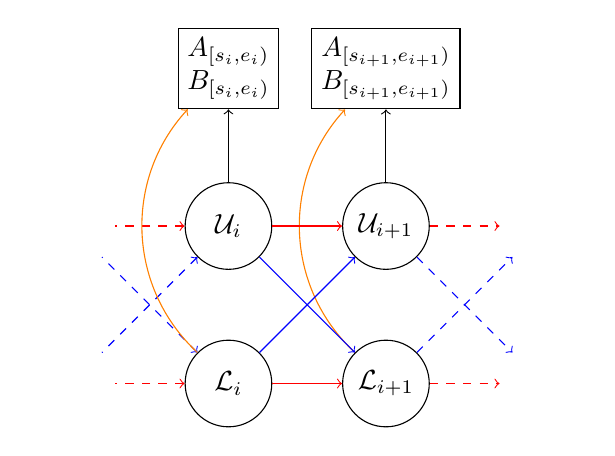
\begin{tikzpicture}
\tikzstyle{circ}=[circle,draw=black,minimum size=11mm]
\tikzstyle{circ_inv}=[circle,minimum size=11mm]
\tikzstyle{square}=[rectangle,draw=black,minimum size=10mm,align=center]
\node [circ_inv] (A0) at (-2,2) {};
\node [circ_inv] (B0) at (-2,0) {};
\node [circ_inv] (A3) at (4,2) {};
\node [circ_inv] (B3) at (4,0) {};
\node [square] (R1) at (0,4) {$A_{[s_i,e_i)}$\\$B_{[s_i,e_i)}$};
\node [square] (R2) at (2,4) {$A_{[s_{i+1},e_{i+1})}$\\$B_{[s_{i+1},e_{i+1})}$};
\node [circ] (A1) at (0,2) {$\mathcal{U}_i$}
edge [<-,dashed,red] (A0)
edge [<-,dashed,blue] (B0)
edge [->] (R1);
\node [circ] (B1) at (0,0) {$\mathcal{L}_i$}
edge [<-,dashed,red] (B0)
edge [<-,dashed,blue] (A0)
edge [->,bend left=45,color=orange] (R1);
\node [circ] (B2) at (2,0) {$\mathcal{L}_{i+1}$}
edge [<-,red] (B1)
edge [->,bend left=45,color=orange] (R2)
edge [->,dashed,red] (B3)
edge [->,dashed,blue] (A3)
edge [<-,blue] (A1);
\node [circ] (A2) at (2,2) {$\mathcal{U}_{i+1}$}
edge [<-,red] (A1)
edge [->] (R2)
edge [->,dashed,red] (A3)
edge [->,dashed,blue] (B3)
edge [<-,blue] (B1);
\end{tikzpicture}
\caption{HMM for assigning absolute phase orientation of each segment. Circles are hidden states; squares are emissions.}
\label{HMMfig}
\end{figure}

After burnin, we take another few MCMC samples and run the aforementioned phasing correction algorithm on each segmentation. This effectively gives us a set of samples $([s_i,e_i),\phi_i)\sim\Phi$ from the posterior distribution $\Phi$ of empirical absolute phase orientations. We can then add a third state to the segmentation MCMC: in addition to proposing that adjacent segments be joined or a given segment be split, we can also choose a region $r_i=[s_i,e_i)$ and phase orientation $\phi_i$ at random from $\Phi$ and flip its phase orientation. If $s_i$ or $e_i$ coincides with a segmentation breakpoint at the current state of the chain, we propose a join; if not, we introduce a new breakpoint at the region boundary and propose a split. The flip is accepted using the same Metropolis criterion as \eqref{metro}, with proposal ratio equal to 1.

\section{Miscellaneous corrections}

\subsection{Reference bias correction}

\subsection{Overdispersion estimation}

Up until now, we have assumed that all uncertainty is \textit{aleatoric} --- all noise on a segment likelihood $\mathcal{L}(f|A_{[s,e)},B_{[s,e)})$ is assumed to come from translating counts $A,B$ to a fraction $f$. However, this is not the only source of noise. 

%name other sources>
%<once we have initial segmentation, we fit beta distribution to counts within each segment; average ratio (weighted by segment lengths)  of sum parameters to fit parameters is overdispersion factor

\section{Non-adjacent segment clustering}

(In-progress)

\noindent Once we have a final set of phase-corrected samples from the distribution over segmentations, we cluster non-adjacent segments using a procedure similar to the MCMC for joining/splitting adjacent segments.

%Now suppose that there are many disjoint segments $\mathcal{S}_j\in\{\mathcal{S}\}$, each with a potentially different allelic imbalance. 
%The total likelihood of a given segmentation is
%\begin{align*}
%\mathcal{L}(\{f\}|\{\mathcal{S}\})=\prod_j \mathcal{L}(f_j|\mathcal{S}_j).
%\end{align*}
%
%We want to find the optimal partition of SNPs (i.e., the optimal set $\{\mathcal{S}\}$)
%
%
%The probability that two allelic segments have the same allelic imbalance is the probability that their beta distribution likelihoods
%\begin{align*}
%f_1\sim \textop{beta}(1 + A_1, 1 + B_1) \qquad f_2\sim \textop{beta}(1 + A_2, 1 + B_2) 
%\end{align*}
%are consistent according to the following two-sided test:
%\begin{align*}
%\textop{Pr}(f_1 \sim f_2) = 2\times\min\lt\{\textop{Pr}(f_1 > f_2),\textop{Pr}(f_1 < f_2)\rt\}.
%\end{align*}
%We could obtain this via convolution, since for $X\sim p$ and $Y\sim q$, we have
%\begin{align*}
%\textop{Pr}(X > Y) = \textop{Pr}(X - Y > 0) = \int_0^\infty d\phi\,\int_{\mathbf{\Theta}} d\theta\,p(\theta)q(\theta - \phi),
%\end{align*}
%but in practice it is cheap enough to obtain via Monte Carlo simulation of the two beta random variables. We draw $n$ samples from $f_1$ and $f_2$ and empirically compute the fraction $\sum_{i=1}^n\bs{1}(f^{(1)}_i > f^{(2)}_i)/n$ for $f_{1\dots n}^{(1)}\sim f_1$ and $f_{1\dots n}^{(2)}\sim f_2$, where $\bs 1$ is the indicator function.
%
%We can sample the posterior probability of segment boundaries via a Metropolis-like sampler. The marginal likelihood of a given set of segments $S$ is
%\begin{align*}
%\mathcal{M}(s) &= \prod_{i\in S} \int_0^1 df\,f^{1 + A_i}(1 - f)^{1 + B_i}\\
%&= \prod_i \beta(A_i, B_i).
%\end{align*}
%We probabilistically propose a new segmentation $S^\ast$ from distribution $q(S^\ast|S)$, and accept $S^\ast$ with probability
%\begin{align*}
%\textop{Pr}(S\to S^\ast) = \min\lt\{1,\frac{\mathcal{M}(S^\ast)q(S|S^\ast)}{\mathcal{M}(S)q(S^\ast|S)}\rt\}
%\end{align*}
%todo: what if $q$ is asymmetric?
%
%For simplicity, let's first assume we have perfect phasing accuracy across an entire chromosome. We initialize each SNP belonging to its own segment. At random, we select two adjacent segments and merge them with probability $p_\text{merge}=\textop{Pr}(f_1 \sim f_2)$, or keep them separate with probability $1 - p_\text{merge}$. If we merge two segments, we compute the marginal likelihood 
%
%\section{Misphasing}
%
%Because we generally do not know perfect phasing information (which would require haplotype-resolved sequencing, e.g., with a parental trio or long reads), we must impute it from a reference panel. Assignment to haplotype $\mathcal{A}$ and $\mathcal{B}$ are therefore not consistent along the entire length of a chromosome arm, but only within small regions (known as ``phase sets'') much smaller than a typical LD block. The SNPs within a given phase set are relative to the haplotypes $\mathcal{A}_i$ and $\mathcal{B}_i$ within that set; we do not know whether $\mathcal{A}_i$ and $\mathcal{A}_j$ belonging to different phase sets are on the same physical molecule.
%
%Furthermore, there is the chance that an individual SNP within a phase set is misphased.
%
%Around a potential phase set boundary, we have four haplotypes $\mathcal{A}_1$, $\mathcal{B}_1$, $\mathcal{A}_2$, and $\mathcal{B	}_2$, with total respective read counts $A_1$, $B_1$, $A_2$, and $B_2$. Suppose the boundary represents a true 
%
%Let $m$ be a binary indicator variable that the break represents a true misphasing. Then by Bayes' rule, the probability of a misphase given the observed readcounts is
%
%\begin{align*}
%p(m|A_1, A_2, B_1, B_2) = \frac{p(A_1, A_2, B_1, B_2|m)p(m)}{\sum_m p(A_1, A_2, B_1, B_2|m)p(m)}
%\end{align*}
%
%Transitions:
%\begin{align*}
%p(f_1 \sim f_2, m|A_1,B_1,A_2,B_2) = p(f_1 \sim f_2|m,A_1,B_1,A_2,B_2)p(m|A_1,B_1,A_2,B_2)
%\end{align*}
%
%\begin{align*}
%f_1 \sim f_2, m=0\\
%f_1 \nsim f_2, m=0\\
%f_1 \sim f_2, m=1\\
%f_1 \nsim f_2, m=1
%\end{align*}
%
%\section{Splitting}
%
%For a given segment comprising $n$ SNPs with total readcounts $A_\mathcal{S}$ on haplotype $\mathcal A$ and $B_\mathcal{S}$ on haplotype $\mathcal B$, the likelihood of breaking it at position $b \in \{1\dots n\}$ is
%\begin{align*}
%\mathcal{L}(b|A_\mathcal{S},B_\mathcal{S}) &= \int_0^1 df\,f^{1 + A_{1\dots b}}(1 - f)^{1 + B_{1\dots b}}\times \int_0^1 df\,f^{1 + A_{b + 1\dots n}}(1 - f)^{1 + B_{b + 1\dots n}}\\
%&= \beta(A_{1\dots b}, B_{1\dots b})\beta(A_{b + 1\dots n},B_{b + 1\dots n})
%\end{align*}
%where $A_{i\dots j}$ is the sum of readcounts from SNP $i$ to $j$ on haplotype $\mathcal A$. The probability of choosing a given $b$ is thus
%\begin{align*}
%p(b|A_\mathcal{S},B_\mathcal{S}) = \frac{\mathcal{L}(b|A_\mathcal{S},B_\mathcal{S})}{\sum_{i=1}^n \mathcal{L}(i|A_\mathcal{S},B_\mathcal{S})}.
%\end{align*}

\end{document}